\documentclass[12pt]{report}
\usepackage[francais]{babel}
\usepackage[utf8]{inputenc}
\usepackage{graphicx}
\usepackage{caption}
\usepackage{amsmath}
\usepackage{hyperref}
\usepackage[section]{placeins}
\addtolength{\hoffset}{-1cm}
\addtolength{\textwidth}{2cm} 
\addtolength{\voffset}{-1cm}
\addtolength{\textheight}{2cm} 


\begin{document}

\begin{titlepage}
\begin{center}

\hfill

\bigskip
\huge{Mémoire  : Projet de Programmation} 
\vfill
\bigskip 
\Huge 
\bigskip Génération automatique de texte \par 
\vfill
\Large Benoît Barthes \par 
		Alexis Boumera \par 
		Baptiste Guiomar \par 
		Claire Pennarun \par 
		Adrien Wintringer
\vfill
\Large Bordeaux 1 \par \Large Projet de Programmation		
		\bigskip 
\bigskip

\Large
\today
\end{center}
\end{titlepage}

\tableofcontents
\newpage

\chapter{Présentation du sujet}

\section{Présentation du domaine}

	Depuis l'apparition des ordinateurs dans les années 50, la question de la reproduction du langage naturel a toujours été une des plus épineuses. \par 
	En effet, le langage humain comprend une multitude de paramètres qui ne sont pas évidents à mettre en oeuvre en termes de programmation : syntaxe, grammaire, intonation, structuration de la pensée... Mais à quoi pourrait bien servir un ordinateur possédant le langage, puisqu'il ne possède pas la pensée, l'intention ; à quoi sert-il de savoir \emph{parler} si l'on ne sait rien \emph{dire} ?

	La question est donc de savoir quoi faire dire à un logiciel, quel texte lui faire générer, et de quelle manière.
	
	La génération




\section{Présentation du projet}

Le logiciel que nous avons développé pendant ce projet permet de générer du texte de manière automatique à partir de données brutes sélectionnées dans une base de données. 

La base de données considérée dans ce projet est une base de données relationnelle, contenant des informations intéressantes pour l'utilisateur, mais non exploitables directement ; il s'agit de données chiffrées, de fonctions, de relations, qui doivent être étudiées avant d'être interprétées.

Ce logiciel peut servir par exemple à analyser automatiquement des données contenues dans une base de données, ou à utiliser ces données intelligemment pour effectuer des tâches répétitives, notamment l'écriture de textes demandant une grande adaptation des termes suivant les situations (on peut penser au mailing automatique pour des commerciaux ou pour une administration, qui doivent adapter leur message à tous les types de destinataires).

\bigskip

La génération du texte se fait à partir de \emph{scénarios utilisateur} : chaque scénario correspond à un but rhétorique visé par l'utilisateur.

Générer de tels textes ne se résumant pas à créer des "textes à trous", notre logiciel permet à l'utilisateur de construire le scénario voulu à partir de \emph{concepts} : ceux-ci peuvent être une action, un événement, une succession, un objet, une personne... Le concept est complètement indépendant de la manière de le représenter (notamment indépendant du lexique utilisé, et même de la langue).

Par exemple, le concept "REUSSIR" peut être représenté ainsi :
$$\begin{bmatrix}
\text{REUSSIR} \\ \text{arg1 = qui\ ?} \\ \text{arg2 = quoi\ ?}
\end{bmatrix}
$$
Les arguments d'un concept peuvent être eux-mêmes des concepts : cela permet de fabriquer des concepts plus complexes.
Par exemple, le concept de causalité prend en argument deux concepts, qui sont eux-mêmes complexes :

$$\begin{bmatrix}
\text{CAUSALITE} \\ \text{arg1 = [antécédent]} \\ \text{arg2 = [conséquence]}
\end{bmatrix}
$$

Les concepts dits "simples" ou atomiques, sont en général les personnes, ou les objets (ce qui correspond souvent aux noms propres ou aux noms communs).

\bigskip

Dans notre projet, le logiciel propose à l'utilisateur de choisir entre la création d'un nouveau scénario (et l'utilisateur devra alors choisir les concepts qu'il veut exprimer, ainsi que leurs arguments) et la réutilisation d'un scénario déjà établi et sauvegardé.

\bigskip

Ce texte est en réalité la sortie du logiciel Syntox, qui est un logiciel développé par M. Lionel Clément, et qui génère du texte grammaticalement et syntaxiquement correct à partir d'une entrée d'une forme spécifique (dite \emph{entrée Syntox} dans notre rapport).

Chaque entrée permet à Syntox de générer toutes les phrases correspondant aux contraintes qui y sont spécifiées.

Par exemple, l'entrée 
$$S [\text{PRED=manger},
    \text{subj=[PRED=grenouille, def=+]},
    \text{obj=[PRED=insecte, def=-]}
]$$
permet de générer :
\begin{enumerate}
    \item la grenouille mange un insecte
    \item la grenouille mange des insectes
    \item les grenouilles mangent un insecte
    \item les grenouilles mangent des insectes
\end{enumerate}
Syntox contient à l'avance une grammaire et un lexique qui correspondent au thème traité. Ces deux composants sont fournis par le client.
Le but de notre logiciel était donc de fournir à Syntox une entrée qui a ensuite été transformée en texte.

\bigskip

Le scénario (c'est-à-dire l'ensemble de concepts plus ou moins complexes que l'utilisateur veut exprimer) est ensuite traité en plusieurs étapes par le logiciel pour générer l'entrée Syntox souhaitée.

Premièrement, le scénario est transformé en un \emph{graphe conceptuel}, c'est-à-dire un graphe acyclique orienté dont les sommets sont des concepts et les arêtes orientées correspondent aux liens entre ces concepts.

Exemple : le graphe conceptuel de "REUSSIR"
\begin{center}
	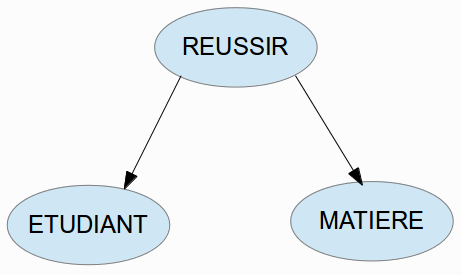
\includegraphics[scale=0.5]{Reussir_graphe.png}
\end{center}

Ce graphe est ensuite parcouru pour le retranscrire en entrée Syntox.
Cette entrée est envoyée au logiciel Syntox, qui génère les phrases correspondantes. On récupère ces phrases, qui correspondent au texte voulu par l'utilisateur. 
Celui-ci peut ensuite enregistrer le résultat dans un fichier.

\bigskip

Notre logiciel comporte deux types d'utilisateurs : l'utilisateur dit "classique", qui ne se préoccupe pas de la manière dont le texte est généré, et l'utilisateur administrateur, qui peut configurer le système.

Ainsi, l'administrateur peut configurer le système (créer les concepts requis et donner les informations de connexion à la base de données), puis l'utilisateur classique n'a plus qu'à utiliser le logiciel, sans avoir besoin de connaître la base de données utilisée ou les détails des concepts qu'il manipule.


\chapter{Etude de l'existant et bibliographie}

\section{Eléments bibliographiques}

L'état de l'art \cite{Bat93} présenté par John Bateman en 1993 (et mis à jour régulièrement depuis) concernant la génération automatique de texte est une base de connaissances très importante pour nous. En effet, l'auteur reprend les avancées des travaux les plus importants dans ce domaine, enrichi d'une grande bibliographie. Il donne également des méthodologies précises pour traiter des problèmes de la génération automatique de texte.
Cet état de l'art, assez conséquent, nous permettra de trouver des références rapidement, même si le sujet que nous traitons n'a pas encore fait l'objet d'une étude poussée.


La synthèse du domaine faite par Laurence Danlos (\cite{Dan00}) est d'un grand intêret pour notre projet. En effet il nous présente de façon très concise ce qu'est la génération automatique de texte. Le premier point intéressant concerne les questions qui se posent généralement dans les applications mettant en oeuvre de la génération de texte, "Quoi dire ?" et "Comment le dire ?". Ce seront probablement des questions que nous aurons à nous poser par la suite. Le document met aussi en avant les différents problèmes et difficultés rencontrés par les sytèmes existants et auxquels nous pourrions avoir à faire face, mais aussi les avantages de tels systèmes. Il est par exemple question de leur "spécialisation" à certains domaines (comme la météo, les finances etc) qui leur permet de ne couvrir qu'une partie de la grammaire et du lexique et d'être ainsi relativement performants. Nous sont aussi présentés dans ce document les différents types d'applications déjà existantes, comme TA(O) (première application développée) ou encore PostGraphe (utilisé dans le domaine statistique). Plus intéressant encore, ce document nous décrit ce que peuvent ou pouraient apporter ces systèmes, comme par exemple une sortie orale (si nous couplions un générateur à une synthétiseur vocal). Une présentation précise des mécanismes et tâches mis en oeuvre dans la génération automatique nous est aussi offerte, avec pour chaque étape une présentation des entrées/sorties. Le document nous présente enfin le problème de l'évaluation de tels systèmes, qui s'avère difficile à résoudre de par leur complexité.

\subsection{EasyText}
Le système de génération de textes EasyText \cite{Dan11} a été développé par Frédéric Meunier, Laurance Danlos, et Vanessa Combet dans le cadre d'une collaboration avec la filliale française Kantar Media de TNS-Sofres. Ce logiciel permet de créer un commentaire à partir d'un tableau de chiffres. 

Contrairement à d'autres procédés de génération de textes tel que les textes à trous ou le publipostage, EasyText utilise un formalisme G-TAG. Ce dernier permet "de transformer une représentation conceptuelle d'un ensemble d'informations en un texte" (d'après Laurence Danlos, \cite {Dan10}). 

\bigskip

Plusieurs étapes ont lieu afin de réaliser le commentaire. Elles se schématisent par deux questions principales: "Quoi dire ?" et "Comment le dire ?" . Dans une première étape il faut sélectionner les informations que l'on peut dire : ce choix se fait en fonction des éléments intéressants présents dans le tableau. On obtient alors une conjonction de formules logiques, qui est ensuite transformée en un texte, en deux temps.

On cherche en premier lieu à transformer la conjonction en phrases (macro-planifi-cation).  On s'appuie alors sur des connaissances rhétoriques et linguistiques de la langue pour structurer l'ordre du texte et déterminer ainsi le "schéma" de la phrase. Enfin, on complète la phrase pour la former selon les conventions de la langue (micro-planification). Pour cela, en fonction du "schéma" auquel elle se rapporte, on ajoute des déterminants, des compléments, etc en prêtant attention à la position à laquelle ils se situent. On s'appuie ici sur des connaissances sémantiques et syntaxiques.  À la suite de toutes ses étapes on obtient un texte formé selon les critères de la langue qui a pour objet les éléments du tableau. 


\section{Etude de l'existant}

\subsection{Projet GAT-2}

Le logiciel GAT-2 (Génération Automatique de Texte 2) \cite{GAT2} est le prédécesseur de notre objectif de travail actuel. Développé l'année dernière par 5 étudiants de master 1 Informatique, il repose principalement sur GAT-1 (développé lui aussi par des étudiants de master 1 Informatique) et sa version améliorée Syntox développée par Lionel Clément: ces deux outils ne se chargent pas du "quoi dire" mais du "comment le dire", prenant en entrée des règles de grammaires énoncées de manière précise et générant un texte fini et syntaxiquement correct.

GAT-2, dans sa version finale, traite simplement une requête SQL énoncée par l'utilisateur (ou plutôt choisie dans une liste prédéfinie par les concepteurs), et y répond via une phrase rédigée en français. Pour ce faire, il se connecte à la base de données, et traite via des opérations logiques simples la requête afin d'en extraire et d'en déduire plusieurs résultats, qui sont formatés de façon à pouvoir être interprétés par GAT-1 qui se charge d'écrire les données répondant à la requête initiale de l'utilisateur en plein texte.
Cependant, il n'arrive pas pleinement à extraire le "sens" (au sens le plus strict du terme) de la base de données, se limitant à la réponse d'une seule question à la fois de manière assez redondante.

\subsection{Syntox}

Syntox \cite{Clem12} est un logiciel développé par Lionel Clément, chercheur au LaBRI dans l'équipe Méthodes Formelles.

Il est défini par son auteur comme un synthétiseur de texte. C'est un type de programme plutôt récent, il en existe donc peu et sont pour la plupart le fait d'universitaires.

Syntox permet de générer du texte à partir de concepts. C'est l'inverse d'un compilateur comme gcc, qui part des feuilles (mot) pour générer une racine. Au contraire l'entrée de Syntox est une racine (comportant un/des concepts) avec laquelle il génère les feuilles. En d'autres termes il ne vérifie pas qu'une phrase est correcte dans un langage donné, mais il crée une phrase correcte dans une grammaire et un lexique défini à partir d'idées.

Syntox ne se limitera donc pas à la génération d'une unique phrase, il doit pouvoir générer des paragraphes entiers. Sa limite principale est dans les reprises sémantiques comme les anaphores, ou les ellipses.
A l'heure actuelle, le projet représente deux ans de travail et fait un peu plus de 12000 lignes de C++.

Son interface utilisateur est faite via un navigateur web pour permettre de porter les efforts sur le programme en lui même et de ne pas perdre du temps à créer des exécutables pour différentes plate-formes. 


\chapter{Cahier des charges}


\section{Scénarios d'utilisation}

\subsection{Scénarios utilisateur}

\subsubsection{Scénario 1}
	\begin{enumerate}
	\item L'utilisateur se connecte en choisissant le mode "utilisateur" ne requérant pas de mot de passe.
			\item Il sélectionne le projet sur lequel il souhaite travailler, et entre le mot de passe de la base de données correspondante (si il y en a un).
            \item Il choisit scénario existant et dans la liste déroulante il choisit celui qui lui convient en fonction de la base de donnée active .
            \item Il clique sur le bouton "Valider" pour lancer l'exécution du logiciel.
            \item L'utilisateur peut alors voir le résultat généré par le logiciel.
            \item L'utilisateur enregistre le résultat dans un fichier texte en appuyant sur le bouton "sauvegarder".
            \end{enumerate}

\subsubsection{Scénario 2}
    \begin{enumerate}
    		\item L'utilisateur se connecte en choisissant le mode "utilisateur" ne requérant pas de mot de passe.
           \item Il choisit "scénario personnalisé" pour pouvoir commencer la création d'un scénario.
           	\item Dans l'écran  de création d'un nouveau scénario, l'utilisateur peut choisir de rajouter ou de modifier les concepts qui composeront son scénario.
            \item Il clique sur le bouton "Générer le texte" dans le menu "Fichier" pour lancer l'exécution du logiciel.
            \item L'utilisateur trouve que le texte généré ne contient pas assez d'informations, ou des informations non pertinentes, il retourne à l'étape de choix des concepts et les modifie pour affiner le résultat en fonction de ce qu'il recherche.
            \item Lorsque le résultat lui convient, l'utilisateur sauvegarde le scénario.
            \item Enfin l'utilisateur enregistre le résultat dans un fichier texte.
            \end{enumerate}


\subsection{Scénarios administrateur}

\subsubsection{Scénario 1}
    \begin{enumerate}
    \item L'administrateur choisit de se connecter en mode "Administrateur" et doit rentrer un login et un mot de passe.
            \item Il choisit de créer un nouveau projet.
            \item Il peut alors entrer le nom du projet, la base de données qui souhaite employer et les identifiants associés.
            \item L'administrateur peut alors commencer la création du projet en choississant les différents concepts qui seront liés à la base de données.
            \item L'administrateur peut alors enregistrer son projet.
            \end{enumerate}

\subsubsection{Scénario 2}   
    \begin{enumerate}
    \item L'administrateur choisit de se connecter en mode "Administrateur" et doit rentrer un login et un mot de passe.
    		\item Il choisit de modifier un projet.
            \item Il choisit le nom du projet à modifier.
            \item L'administrateur s'attelle à l'association de requêtes SQL avec des concepts nouveaux qu'il crée.
            \item L'administrateur enregistre le projet.
            \end{enumerate}


\section{Besoins fonctionnels}

\subsection{Besoins utilisateur}

L'utilisateur classique doit pouvoir effectuer plusieurs actions de manière assez intuitive. Nous proposerons donc une interface graphique pour accéder aux diverses fonctionnalités.

	\begin{itemize}
	\item Dans un premier temps, l'utilisateur pourra sélectionner la base de données sur laquelle il souhaite travailler.
	\item L'utilisateur doit pouvoir créer un nouveau scénario ou charger un scénario pré-existant.
	\item Lors de la création d'un nouveau scénario, les différents concepts seront sélectionnés et une vue globale du scénario sera proposée à l'utilisateur.
	\item La visualisation du texte généré se fera via l'interface graphique.
	\item Le résultat pourra être enregistré dans un fichier .txt dont le nom sera choisi par l'utilisateur. Ce fichier lui permettra de réutiliser le texte généré à sa guise.
	\end{itemize}

\subsection{Besoins administrateur}

L'administrateur est un utilisateur avancé qui peut configurer les différentes étapes de la génération du texte. Il possède un mode différent de celui de l'utilisateur classique dans l'interface graphique.

\subsubsection{Besoins généraux}

L'administrateur doit pouvoir:

\begin{itemize}

\item Lier les concepts à la base de données (par des requêtes SQL) via une interface graphique ;
\item Choisir des concepts pertinents selon la base de données utilisée. L'administrateur va alors lier à chaque concept une ou plusieurs requêtes SQL nécessaire à son expression;
\item Il a les mêmes besoins que l'utilisateur classique, et doit pouvoir accéder aux mêmes informations;
\item Il doit pouvoir visualiser le texte final, afin de pouvoir le vérifier et éventuellement modifier l'étape de liaison concepts/requêtes en cas de non-satisfaction.
\end{itemize} 

\subsubsection{Besoins liés à la base de données}

D'un point de vue "administration de la base de données", l'administrateur doit pouvoir effectuer les actions suivantes :

\begin{itemize}

\item Ajouter des informations de connexion à une base de données;
\item Modifier les configurations de la base de données, ou changer son emplacement, ainsi que lui associer des profils utilisateur (identifiant/mot de passe);
\item Vérifier le bon fonctionnement et retour des requêtes SQL utilisées;
\item Tester les requêtes directement sur le logiciel afin de vérifier leur bon fonctionnement.
\end{itemize} 

\subsubsection{Besoins liés aux concepts et aux scénarios}

\begin{itemize}
\item \emph{Créer/modifier/visualiser/supprimer des concepts}

	Un concept étant un objet comprenant un nom (le nom du concept lui-même) et des arguments d'un nombre et d'un type précis, l'administrateur doit pouvoir entrer de nouveaux concepts dans la liste des concepts.
	La visualisation des concepts correspond à la visualisation du graphe conceptuel qui lui est associé.
	
\item \emph{Créer des scénarios}

	L'administrateur doit pouvoir créer de nouveaux scénarios qui seront proposés à l'utilisateur s'il choisit de charger un scénario pré-enregistré.
	
\end{itemize}


Le client (M. Lionel Clément) se chargera de la génération du lexique et de la grammaire associée au logiciel Syntox, il nous fournira également les concepts dont nous aurons besoin.

\subsection{Besoins système}

Indépendamment des besoins fonctionnels de l'utilisateur classique et de l'utilisateur administrateur, nous avons des besoins fonctionnels relevant du système. Parmi ces besoins on trouve :

\subsubsection{Interface graphique}

Pour répondre aux besoins des utilisateurs classiques et administrateurs, l'interface graphique aura pour fonction la création de l'entrée Syntox. Cette création du point de vue de l'utilisateur consistera à choisir, par le biais d'éléments graphiques, les concepts qu'il souhaite employer dans le texte final. Il pourra choisir les concepts et leurs arguments, qu'ils soient simples ou complexes.

\bigskip

La fenêtre qui permettra la création de l'entrée Syntox - fenêtre de création - sera commune à l'utilisateur classique et à l'administrateur. Tous deux ont les mêmes besoins pour cet aspect du programme, il n'est donc pas nécessaire de la dissocier.

\bigskip

L'utilisateur administrateur aura accès à une fenêtre spécifique, consacrée à la gestion des concepts et des éléments de la base de données. Son rôle en tant qu'administrateur est  de relier les concepts à des requêtes. Au moyen de cette fenêtre il pourra répondre à ce besoin fonctionnel.

\subsubsection{Génération de requêtes SQL}

On doit prévoir un module capable de communiquer avec la base de données au moyen de requêtes SQL: on doit donc être capable de les envoyer, et de recevoir la réponse de la base de données, ainsi que de traiter ces réponses pour pouvoir les utiliser.

\subsubsection{Base de données}

Nous avons besoin de pouvoir nous connecter à une base de données en lecture afin de pouvoir lire sa structure en lui soumettant des requêtes SQL. Pour le moment nous ne nous limitons pas à l'utilisation d'une seule base de données, afin de pouvoir étudier l'utilisation de différents concepts sur d'autres données.

Nous envisageons de stocker les concepts dans une base de données indépendante de celle où se trouvent les données initiales, pour pouvoir la transporter sans véhiculer l'ensemble des données.

\subsubsection{Création du graphe conceptuel}

Pour la création du graphe conceptuel, nous aurons besoin d'une librairie de graphes:
nous devons pouvoir afficher le graphe, le modifier, le stocker en mémoire et le parcourir.

Ce graphe étant un graphe orienté acyclique, le parcourir pour générer l'entrée Syntox sera assez simple (un parcours en profondeur classique, en marquant les sommets déjà explorés).
  
\subsubsection{Création de la requête pour Syntox}

Il s'agira ici de transformer le graphe conceptuel obtenu précédemment en entrée Syntox avec sa syntaxe spécifique. On créera dans ce but une table de correspondance entre chaque concept et l'entrée Syntox correspondante, qui sera modifiable par l'administrateur.

\subsubsection{Génération de phrases}

On utilisera Syntox afin de générer les phrases à partir de l'entrée créée par notre programme.
On devra alors soit intégrer Syntox dans notre programme afin de lui communiquer directement les entrées, et les récupérer pour les stocker dans un fichier; soit établir un protocole de communication avec la version en ligne de Syntox fonctionnant dans les deux sens: l'envoi de l'entrée et la récupération des phrases générées par Syntox.

\section{Besoins non-fonctionnels}

Afin d'être conforme aux spécifications fournies par le client, le logiciel devra répondre à un certain nombre de besoins non-fonctionnels.

\subsection{Génération d'une entrée Syntox}

\begin{itemize}
	\item Le but premier du logiciel est de générer une entrée Syntox. Nous devons donc faire en sorte que cette entrée soit de forme compatible avec le logiciel Syntox. Pour ce faire nous devrons avoir en mémoire un ensemble de règles qui relieront chaque concept exprimé au formalisme Syntox correspondant.
	\item L'entrée Syntox que le logiciel génèrera devra permettre la production d'une phrase grammaticalement correcte par Syntox, ce qui sera assuré par une construction soignée et précise de l'entrée.
\end{itemize}


\subsection{Facilité d'utilisation}

Le logiciel est conçu selon les besoins de notre client. Nous ne
savons pas si d'autres personnes l'utiliseront. Nous partons donc avec
l'objectif d'avoir un logiciel utilisable par une personne ayant des
connaissances basiques en informatique. Cependant, il est à noter que
pour l'administrateur, des connaissances minimales en base de données sont
souhaitées.

\subsection{Portabilité}

Nous développons sous Linux et notre client utilise MacOs X, cela
nécessite que notre programme soit le plus portable possible.
Pour passer le moins de temps possible à compiler notre logiciel pour
différentes plateformes ; l'utilisation d'une machine virtuelle est de
ce fait nécessaire.
Nous utiliserons l'environnement Java qui permet de combiner portabilité
et simplicité.
L'unique contrainte est Syntox mais il est utilisé via le réseau, donc
il ne doit pas être compilé spécifiquement pour la machine de
l'utilisateur final.

\subsection{Besoins relatifs aux bases de données utilisées}
  
Pour les bases de données sur lesquelles on travaillera, on se limitera
aux bases relationnelles (SQL) car elles sont les plus répandues et
permettent donc un travail sur des thèmes plus diversifiés. Cela
permettra également de disposer de plus d'outils pour les manipuler de
par le nombre de librairies disponibles et d'un langage connu et normé,
par rapport à des bases de données non SQL (souvent utilisées pour
l'entrepôt de données comme les bases de données MongoDB) dont les
outils sont moins accessibles. Dans le cas de bases de données non SQL,
chaque base de données développe son propre langage, rendant la lecture
par le même logiciel de plusieurs de ces bases impossible, ce qui ne les
rend pas intéressantes dans le cadre de notre projet.

En conclusion nous nous limiterons pour l'instant à une base de données
MySQL, car il s'agit des plus répandues. En parallèle, on s'occupera de
rendre notre logiciel adaptable au maximum à des bases de données
relationnelles autres que MySQL, afin de rendre possible une extension
du programme dans le futur.

Concernant le travail sur la base de données, on se contentera tout
d'abord de connexions publiques (sans mot de passe) pour l'envoi des
requêtes. On veut avant tout ne pas avoir à gérer un stockage de mot de
passe car cela poserait des problèmes de sécurité (cryptage etc).
On doit donc pouvoir effectuer des requêtes sur la base de données en
tant que simple utilisateur, car on aura pas la possibilité d'une
connexion en tant qu'administrateur.

En ce qui concerne les besoins internes à notre logiciel, il nous semble
que l'utilisation d'une base de données est superflue.  


\chapter{Architecture}

\section{Diagrammes et schémas}

Ils schématisent les interactions entre le programme, l'utilisateur et l'administrateur, avec la base de données et Syntox.

Avant tout, l'administrateur crée des concepts: ces concepts sont primordiaux pour la production finale de texte et régissent la manière dont est interrogée la base de données.

Il configure ensuite la connexion avec la base de données. Il se charge de la mise en place des requêtes SQL, et de leur association avec des concepts existants.

Il se doit de compléter la grammaire (s'il en existe une) et d'enrichir le lexique pour répondre aux concepts que l'on souhaite expliquer; autrement dit, chaque base de données aura besoin de son propre lexique et éventuellement d'un ajustement de la grammaire pour obtenir un résultat satisfaisant.

L'utilisateur peut alors sélectionner un scénario ou interroger la base de données avec les outils proposés par l'IHM. Ses actions vont donner aux programmes les paramètres nécessaires à la création d'une entrée Syntox, après la récupération des informations nécessaires via des requêtes SQL. Syntox est alors sollicité pour générer un texte final.

A l'heure actuelle, on ne sait pas encore si le résultat final sera consultable uniquement via Syntox ou renvoyé à l'utilisateur via notre logiciel.

\subsection{Diagramme de cas d'utilisation}

	Ce diagramme présente les fonctionnalités accessibles à l'utilisateur classique et à l'administrateur.

	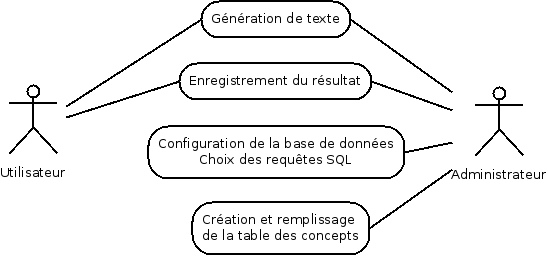
\includegraphics[scale=0.5]{Diagramme1.png}

\subsection{Schémas de fonctionnement}

	\subsubsection{Schéma de fonctionnement - Utilisateur}
	Le schéma suivant décrit le fonctionnement du logiciel du point de vue d'un utilisateur lambda.
	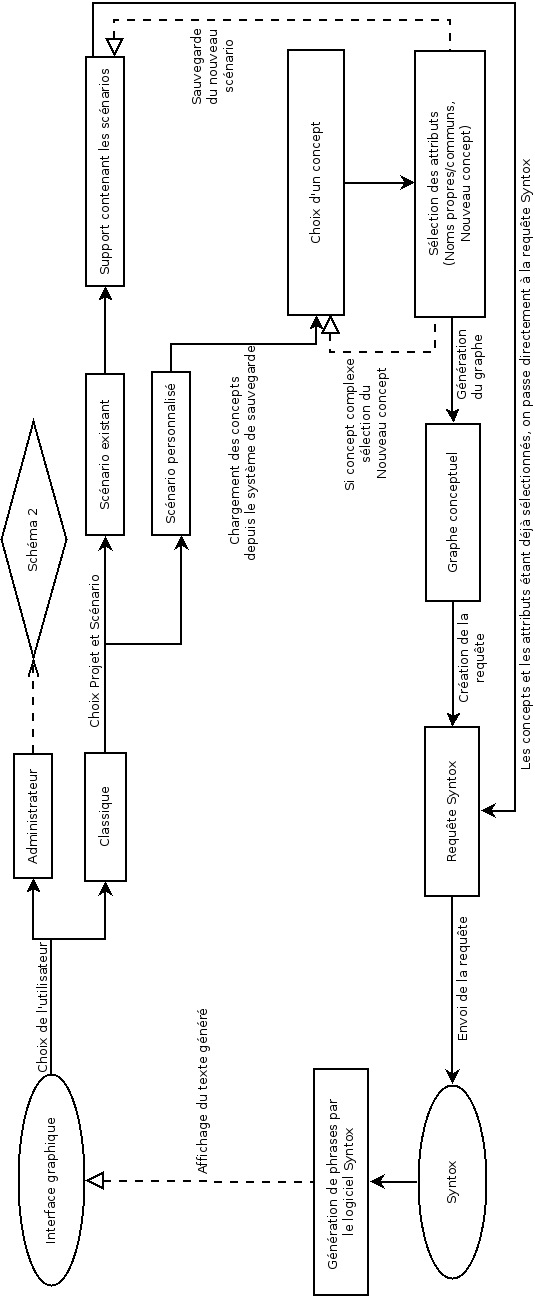
\includegraphics[scale=0.45]{FonctionnementUtilisateur.png}
	

	\subsubsection{Schéma de fonctionnement - Administrateur}
	Le schéma suivant décrit le fonctionnement du logiciel du point de vue d'un administrateur.
	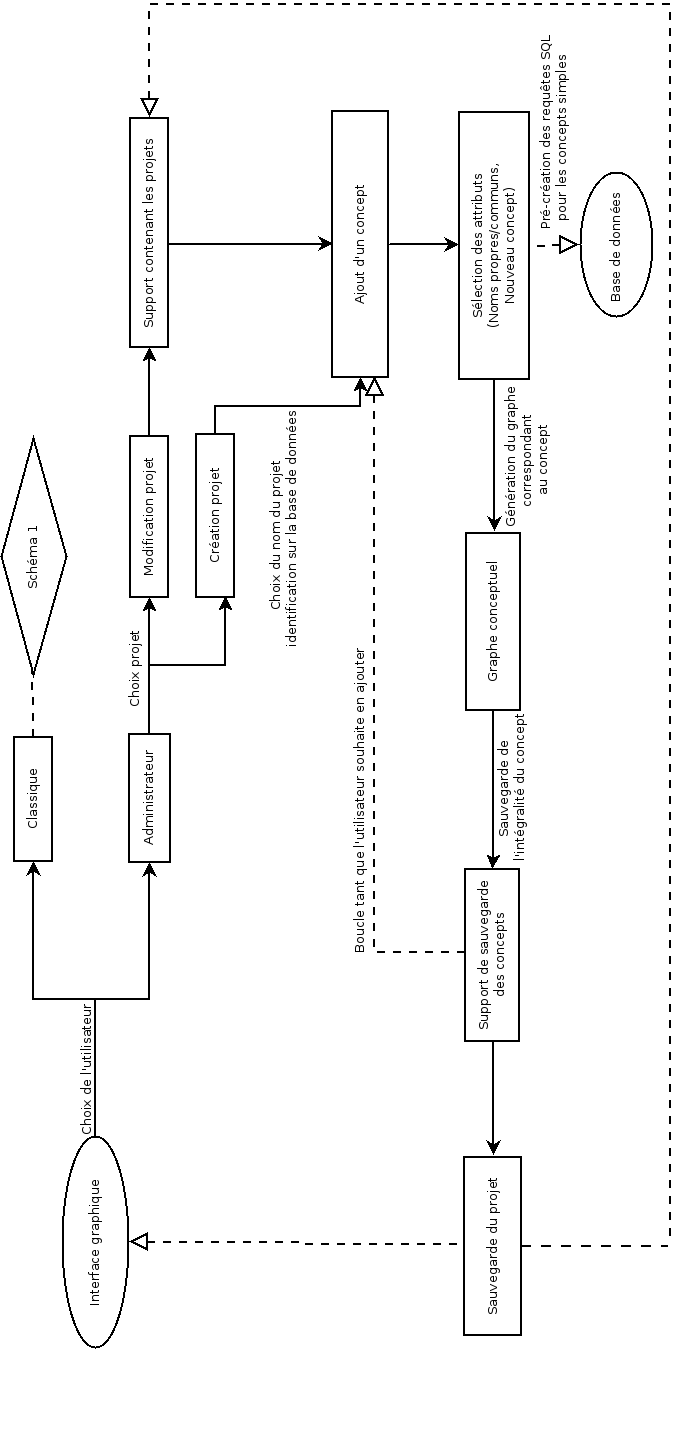
\includegraphics[scale=0.45]{FonctionnementAdministrateur.png}

\subsection{Diagramme de séquence}

	Ce diagramme de séquence explicite les étapes de configuration de la base de données, du lexique et de la grammaire par l'administrateur. 

	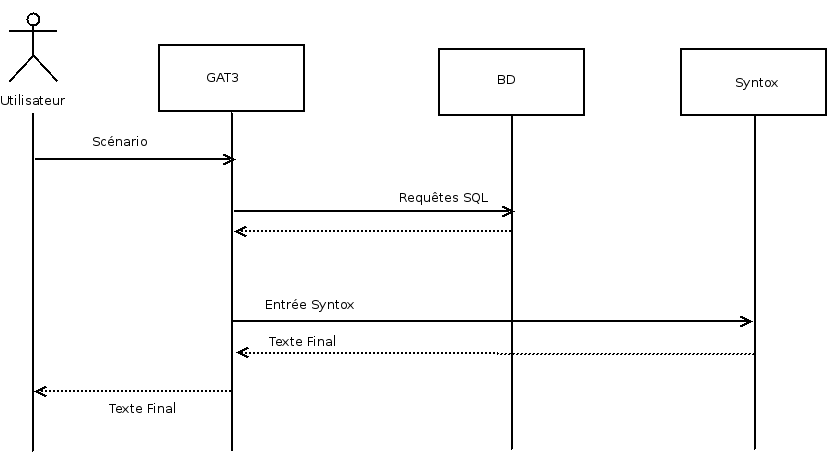
\includegraphics[scale=0.4]{diasequence2.png}


\section{Architecture}
Notre programme se composera de cinq packages principaux: Database, Linguistic, FileManager, SyntoxConnection et IHM, correspondant aux différentes fonctionnalités du programme.
Chacun de ces packages comportera les classes nécessaires à son bon fonctionnement.

\subsection{Diagramme de packages}
Le diagramme suivant présente la structure générale du logiciel.

\begin{figure}[!h]
\begin{center}
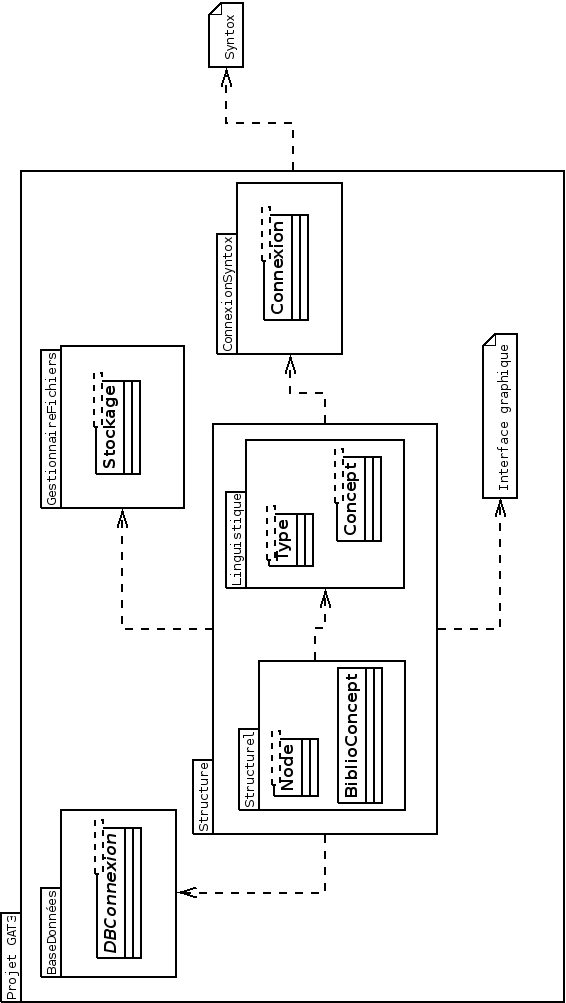
\includegraphics[scale=0.45]{DiagPackages.png}
\caption{Diagramme de packages}
\end{center}
\end{figure}



\subsection{Diagrammes de classes}

\begin{figure}[h!]
\begin{center}
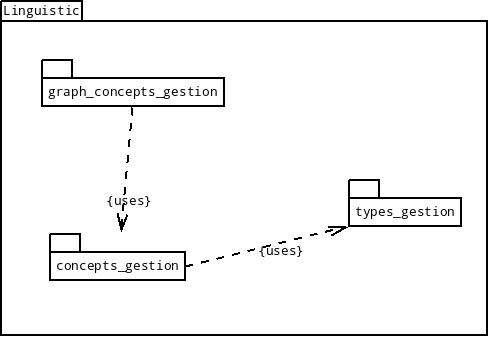
\includegraphics[scale=0.5]{DiagLinguisticPackages.png}
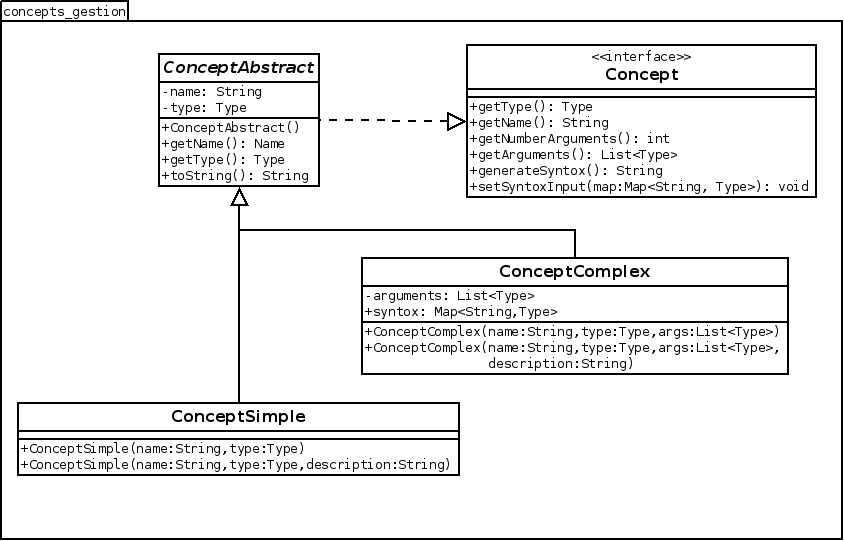
\includegraphics[scale=0.5]{DiagLinguistic_concepts_gestion.png}
\caption{Diagramme du package Linguistic et diagramme de classes du sous-package concepts\_gestion}
\end{center}
\end{figure}

\begin{figure}[h!]
\begin{center}
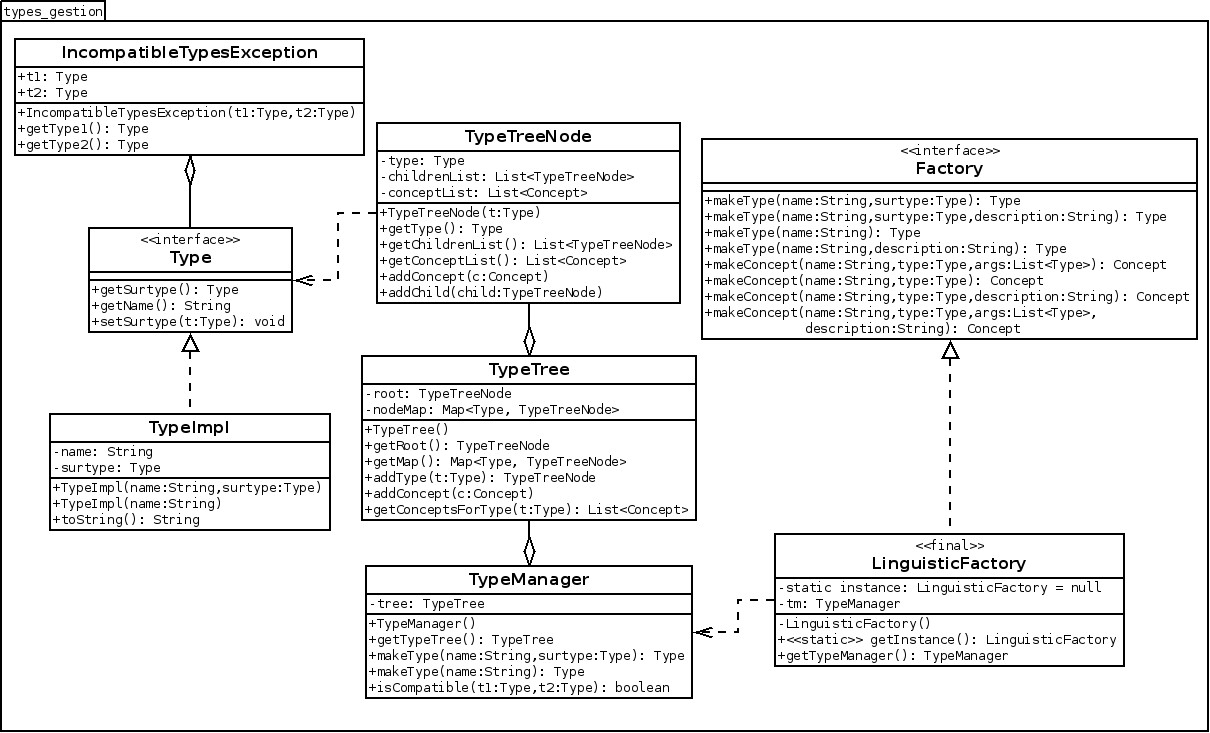
\includegraphics[scale=0.4]{DiagLinguistic_types_gestion.png}
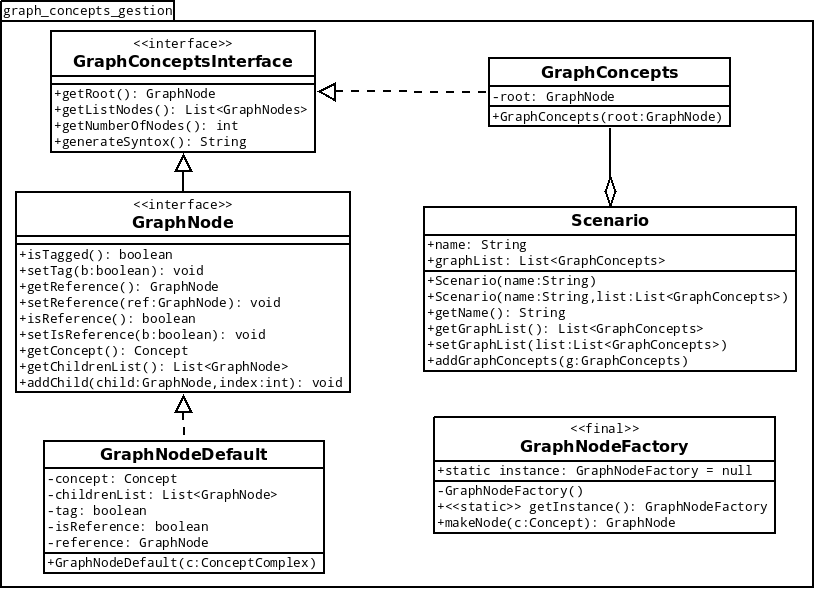
\includegraphics[scale=0.5]{DiagLinguistic_graph_concepts_gestion.png}
\caption{Diagramme de classes des sous-packages types\_gestion et graph\_concepts\_gestion}
\end{center}
\end{figure}

\begin{figure}[h!]
\begin{center}
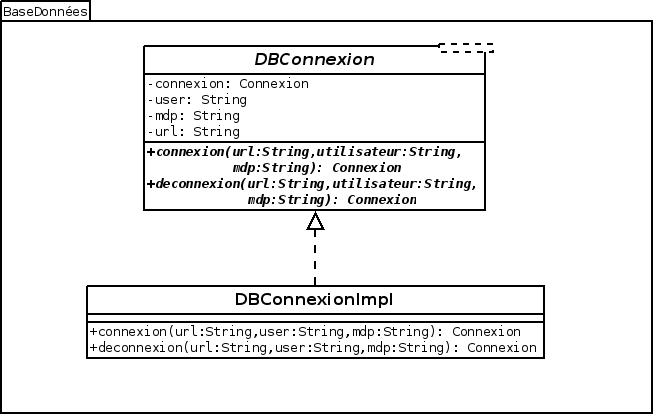
\includegraphics[scale=0.5]{DiagBD.png}
\caption{Diagramme du package BaseDonnées}
\end{center}
\end{figure}

\begin{figure}[h!]
\begin{center}
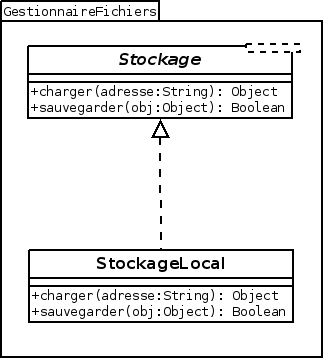
\includegraphics[scale=0.5]{DiagStockage.png}
\caption{Diagramme du package GestionnaireFichiers}
\end{center}
\end{figure}


\begin{figure}[h!]
\begin{center}
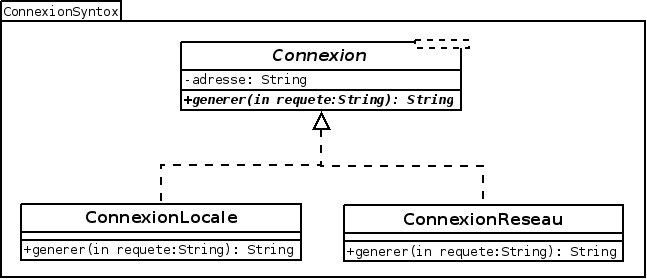
\includegraphics[scale=0.5]{DiagSyntox.png}
\caption{Diagramme du package ConnexionSyntox}
\end{center}
\end{figure}

\FloatBarrier

\subsection{Diagrammes de séquence}


\begin{figure}[h!]
\begin{center}
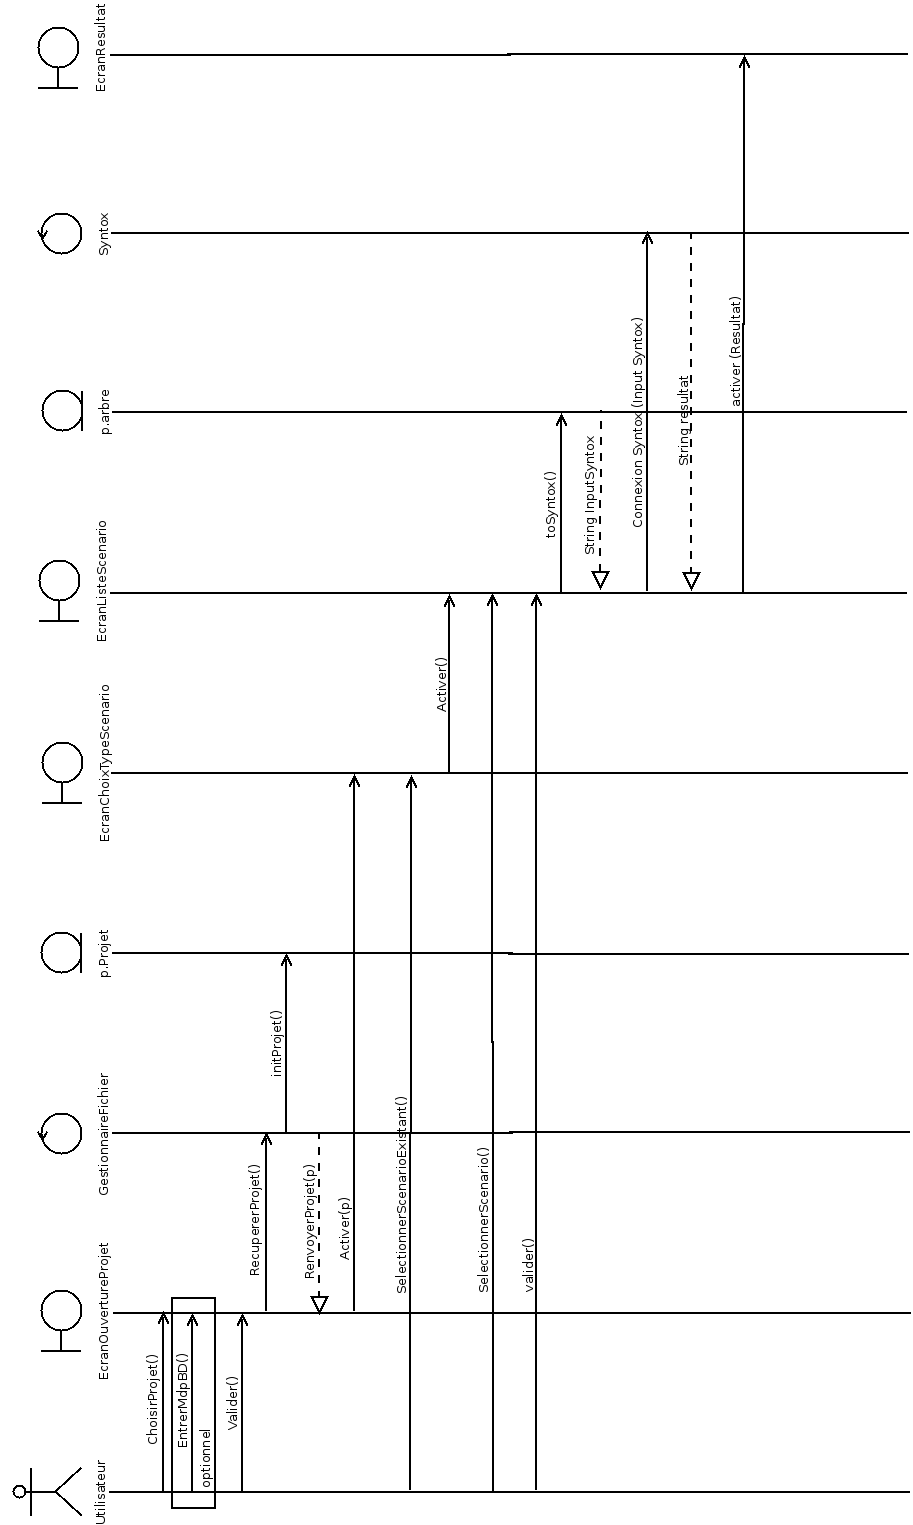
\includegraphics[scale=0.34]{DiagSeq.png}
\caption{Diagramme de séquence Scénario 1}
\end{center}
\end{figure}


\begin{figure}[h!]
\begin{center}
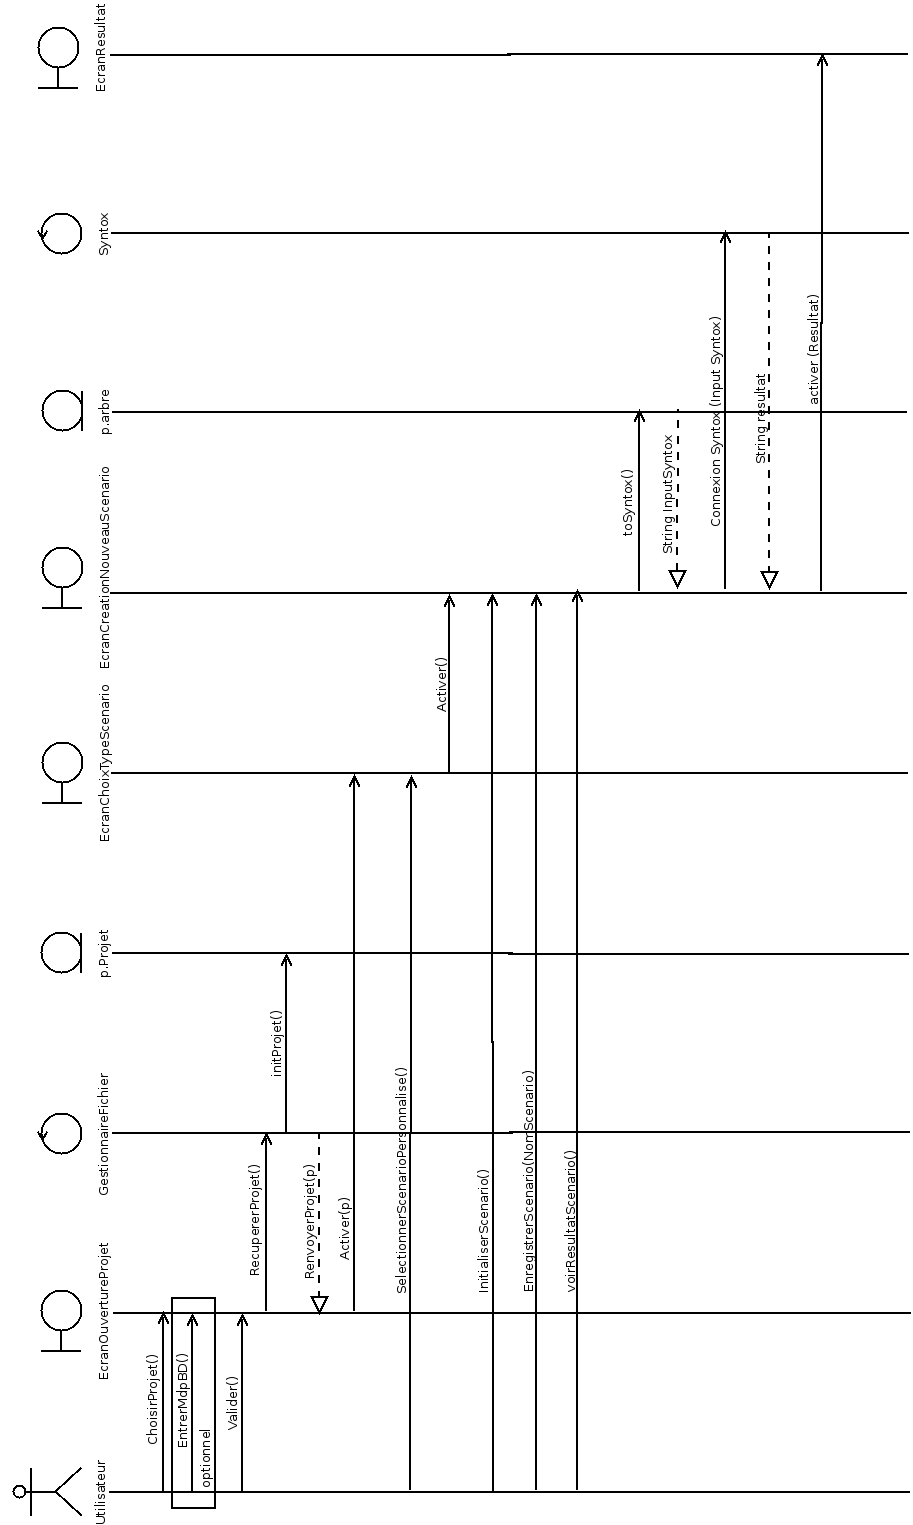
\includegraphics[scale=0.34]{DiagSeq2.png}
\caption{Diagramme de séquence Scénario 2}
\end{center}
\end{figure}


\begin{figure}[h!]
\begin{center}
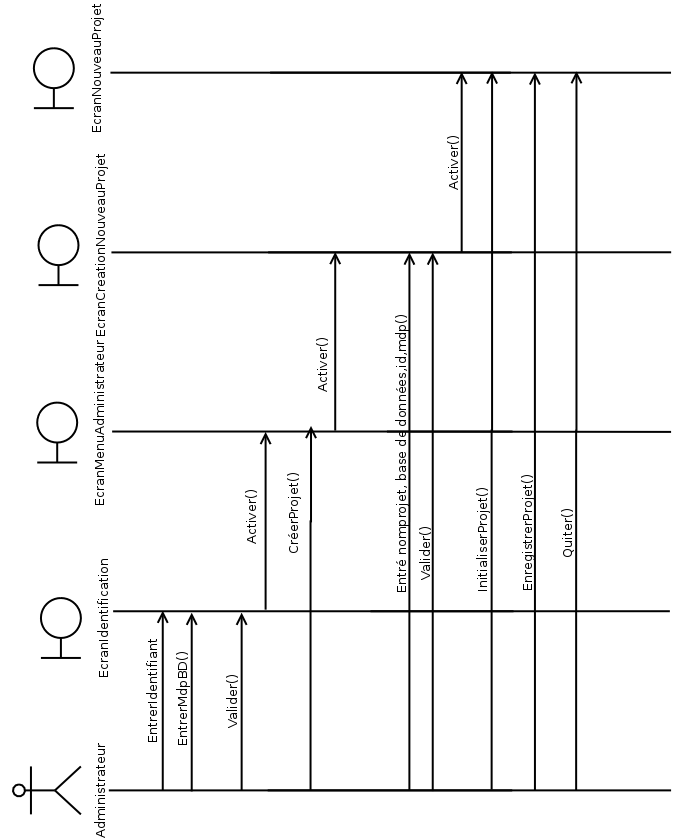
\includegraphics[scale=0.34]{DiagSeq3.png}
\caption{Diagramme de séquence Scénario 3}
\end{center}
\end{figure}


\section{Justifications}

% A VOIR SI NECESSAIRE, SI OUI, OU LE PLACER ?

\subsubsection*{Package Structure}
Il est composé de deux sous-packages, Structurel et Linguistique :

\begin{itemize}
\item Le package Structurel contient tous les objets de modélisation d'arbres.
\item Le package Linguistique contient les objets liés à la manipulation du langage: concepts et types des concepts.
\end{itemize}

\subsubsection*{Package Linguistique}
\begin{itemize}
\item Interface Concept : Dans cette interface se trouveront toutes les fonctionnalités liées aux concepts.

\item Interface Type : Cette interface sera utilisée afin de regrouper plusieurs concepts sous un même type. 

\item Classe ConceptImpl: Cette classe permet de factoriser du code entre les différentes implémentations de la classe Concept.

\item Classe ConceptAtomique: Il s'agit de l'implémentation d'un concept directement relié à une ligne d'une table de la base de données, c'est à dire qu'elle contient uniquement une requête SQL et pas un autre concept.

\item Classe ConceptComplexe: Il s'agit de l'implémentation d'un concept dont les arguments sont d'autres concepts, atomiques ou complexes.

\item Classe TypeConcept: Cette classe contient l'implémentation de l'interface Type.
\end{itemize}

\subsubsection*{Package Structurel}
\begin{itemize}
\item Interface Node: Dans cette interface sont présentées les fonctionnalités nécessaires à la réalisation d'un schéma de phrase.

\item Classe NodeConcret: Implémentation de l'interface Node.

\item Classe BiblioConcept: Classe visant à organiser tous les concepts en les regroupant par type à des fins de recherche (facilité d'accès).

\item Classe BiblioScenario: Cette classe regroupe l'ensemble des scénarios d'un projet. Cette classe sera utilisée lorsque l'utilisateur cherchera un scénario à utiliser. Chaque création de scénario fera appel à cette classe.

\item Classe BiblioProjet: Contient les informations de connexion à la base de données, une bibliothèque de concepts, une bibliothèque de scénarios pour chacun des projets.
\end{itemize}

\subsubsection*{Package BaseDonnées}
Interface DBConnexion: Cette interface sera implémentée par DBConnexionImpl. Elle contient les outils nécessaire à la connexion aux bases de données.

\subsubsection*{Package GestionnaireFichiers}
Interface Stockage: Permet toutes les actions basiques liées à la manipulation des données volatiles.

\subsubsection*{Package ConnexionSyntox}
Interface Connexion: Contient les fonctionnalités permettant de communiquer avec le logiciel Syntox.

\subsubsection*{Package InterfaceGraphique}
Ce package contiendra tous les éléments de l'interface graphique et des fenêtres.



\chapter{Implémentation}

\section{Algorithmique et structures de données utilisées}

\section{Communication avec la base de données}

\section{Package Linguistique}

\section{Génération de l'entrée Syntox}





\section{Autres}



\section{Problèmes rencontrés et remarques}

\chapter{Présentation du logiciel fourni}

% Explications et présentation de l'IHM
\begin{figure}
\centering
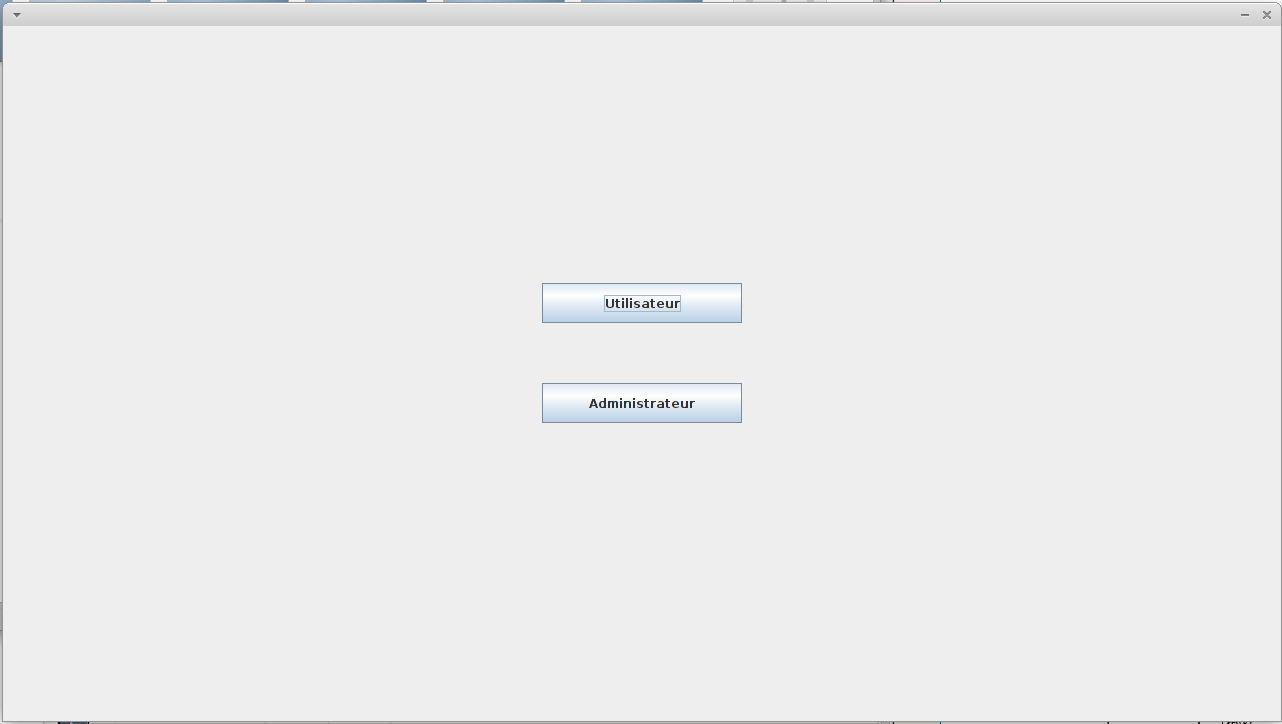
\includegraphics[scale=0.3]{IHM/accueil.png}
\caption{Ecran de connexion}
\end{figure}

\begin{figure}
\centering
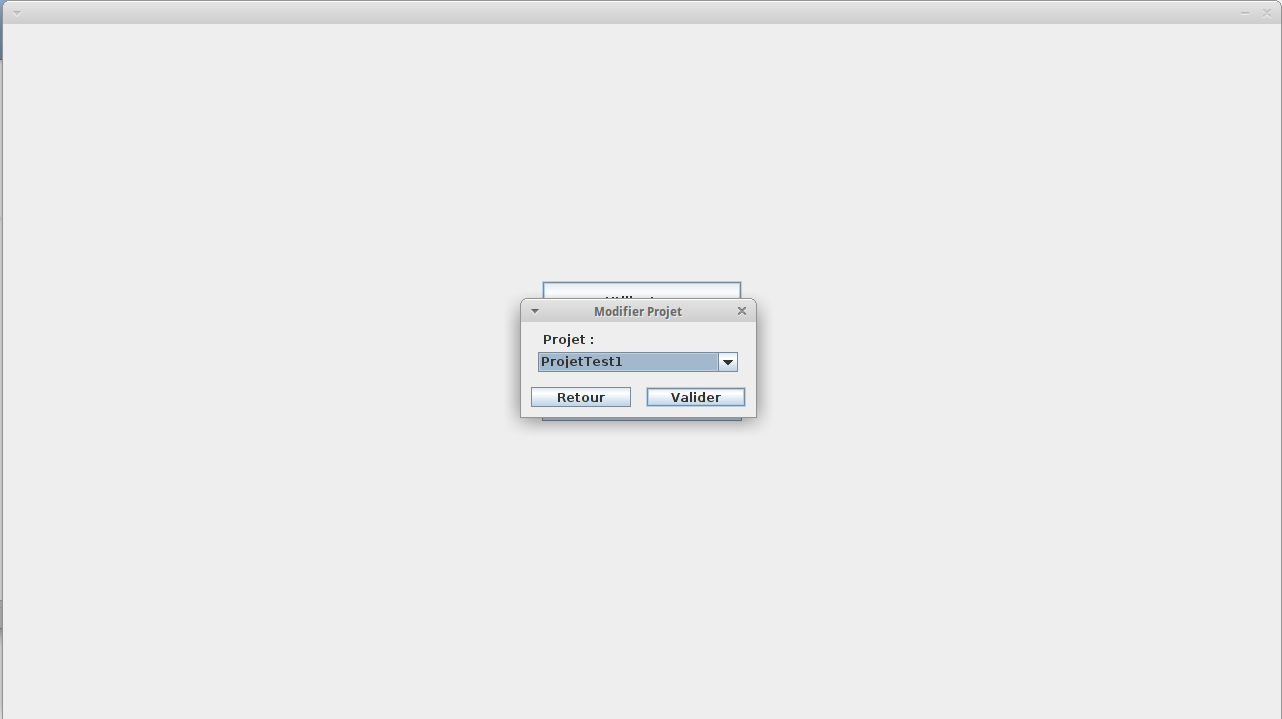
\includegraphics[scale=0.3]{IHM/selection_modifier_projet.png}
\caption{Ecran d'ouverture d'un projet}
\end{figure}

\begin{figure}
\centering
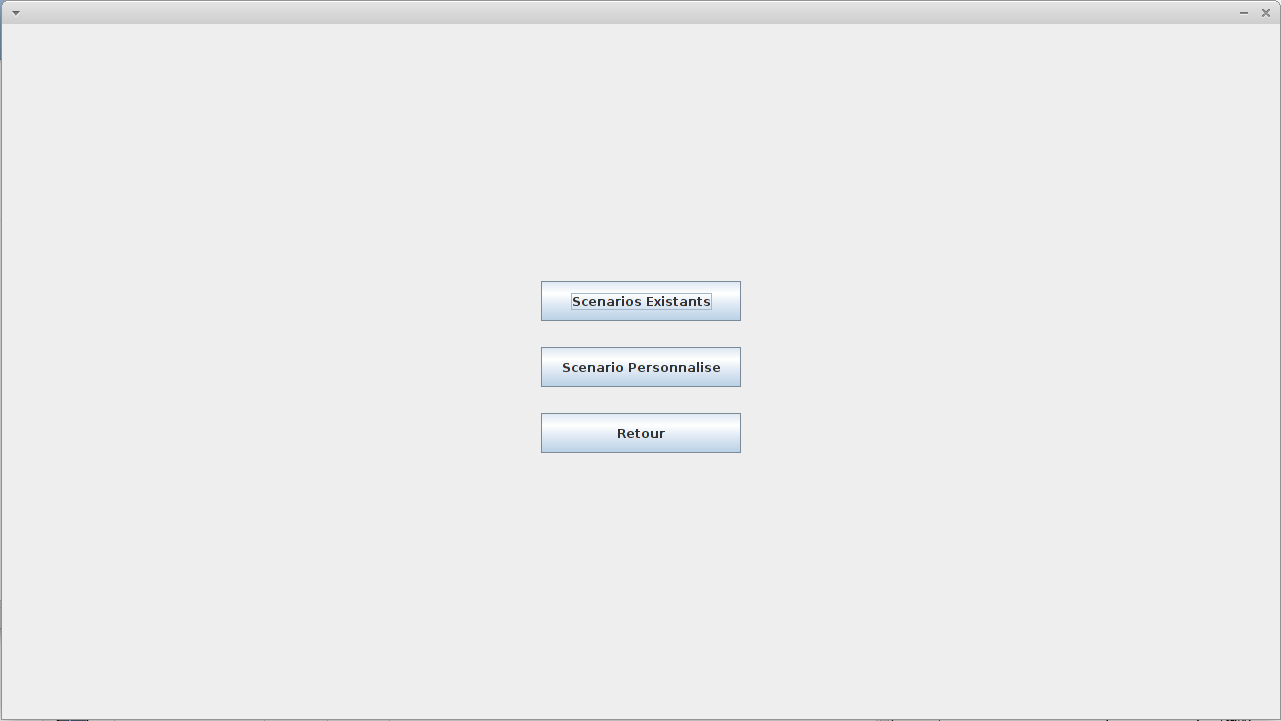
\includegraphics[scale=0.3]{IHM/choix_scenario.png}
\caption{Ecran de sélection de scénario existant/personnalisé}
\end{figure}
\begin{figure}
\centering
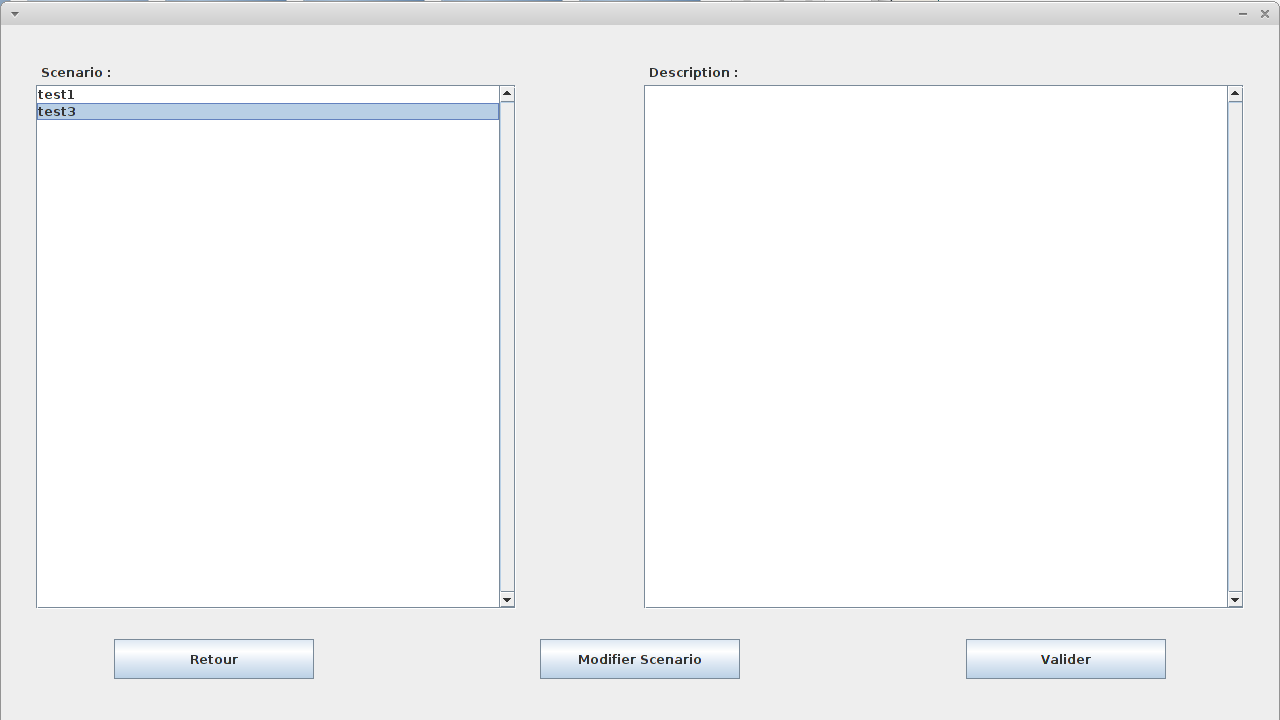
\includegraphics[scale=0.3]{IHM/selection_scenario.png}
\caption{Ecran de sélection de scénario existant}
\end{figure}
\begin{figure}
\centering
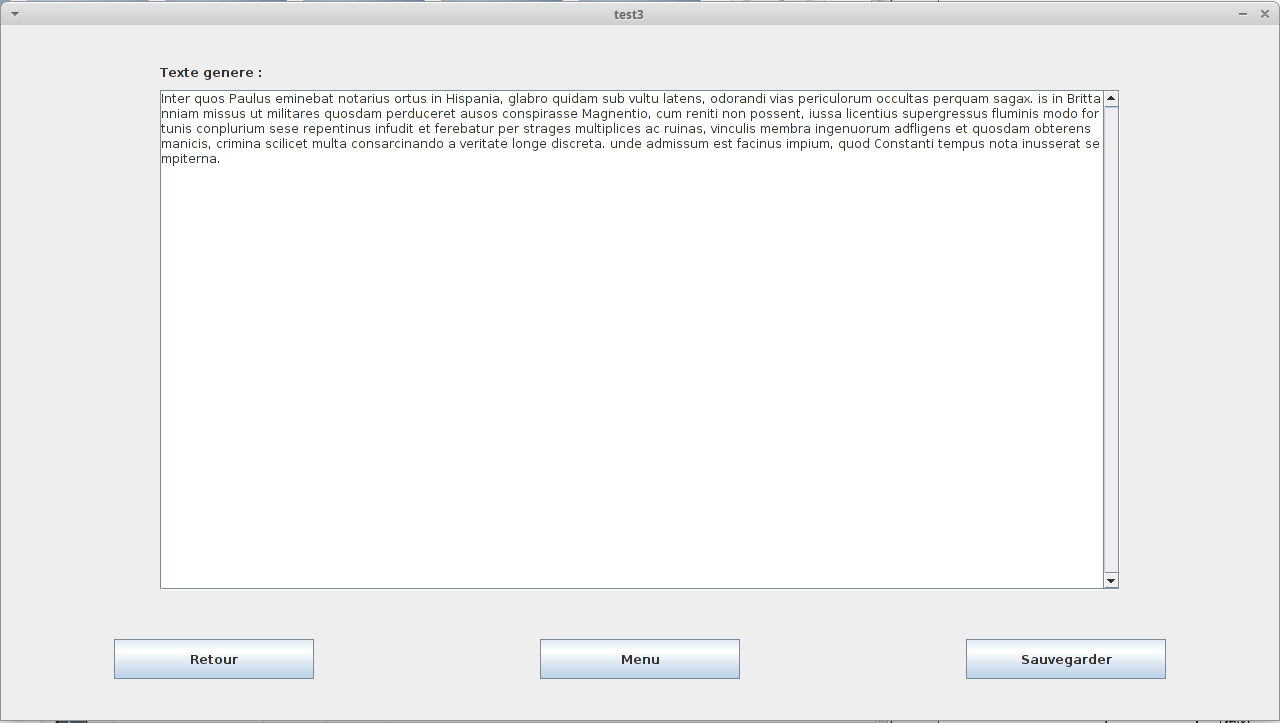
\includegraphics[scale=0.3]{IHM/affichage_resultat.png}
\caption{Ecran affichant le texte généré}
\end{figure}
\begin{figure}
\centering
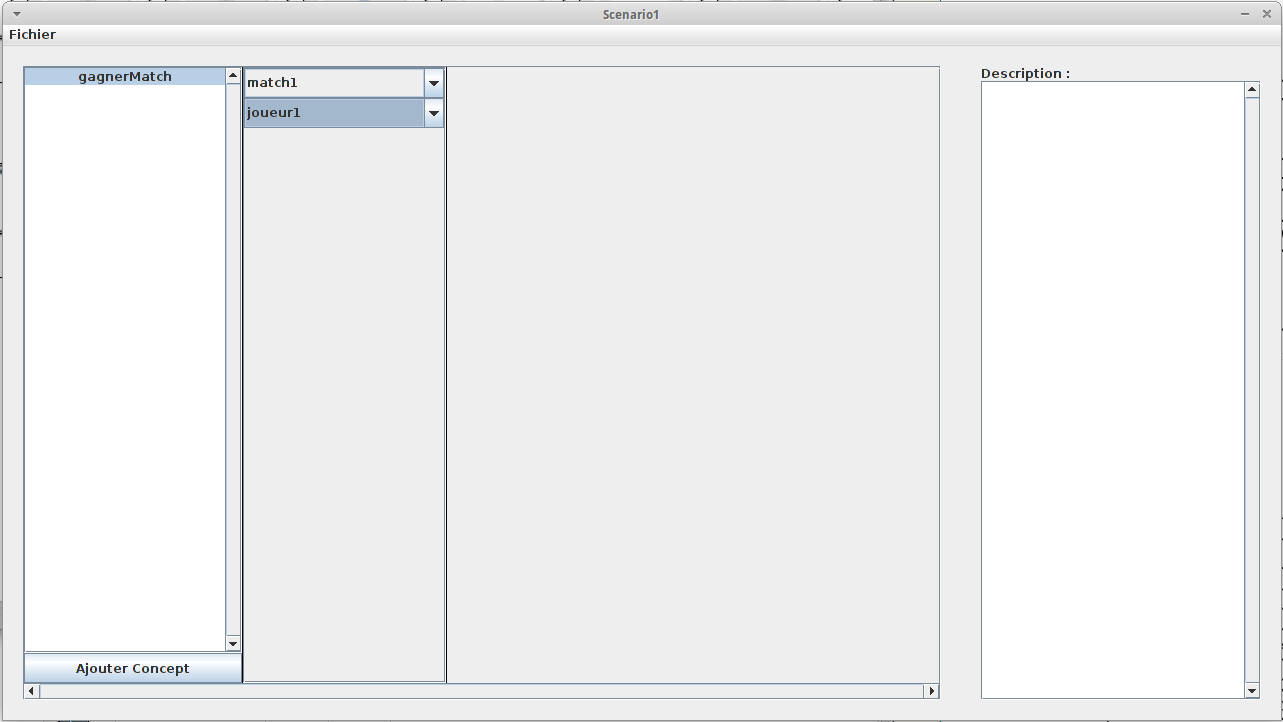
\includegraphics[scale=0.3]{IHM/remplissage_scenario.png}
\caption{Ecran de création d'un nouveau scénario}
\end{figure}
\begin{figure}
\centering
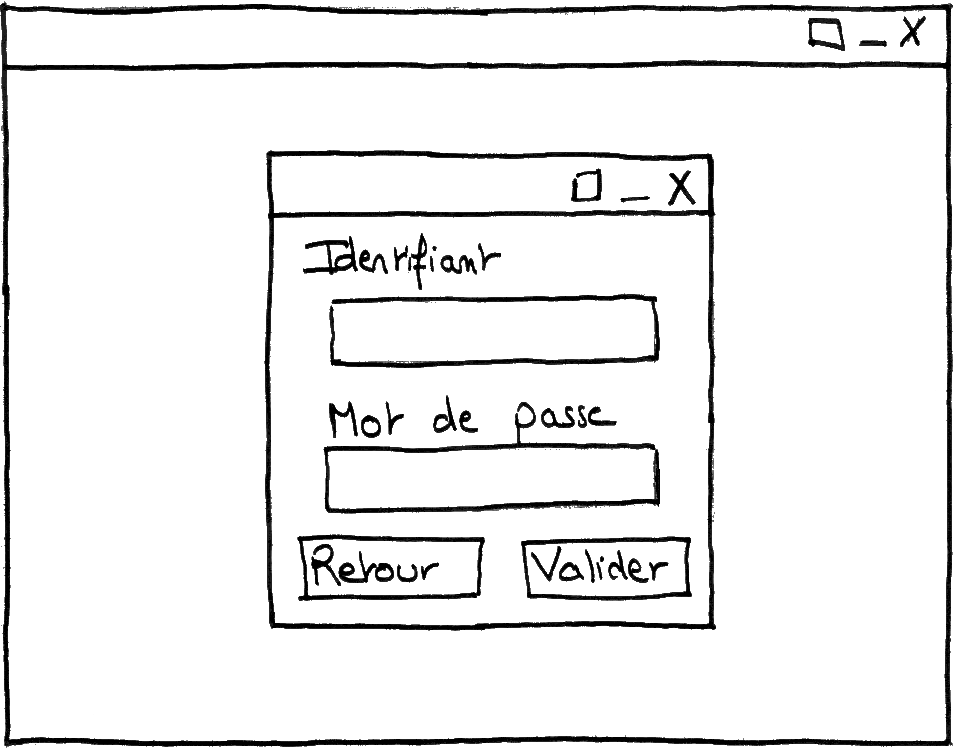
\includegraphics[scale=0.5]{IHM_5b.png}
\caption{Ecran de connexion à la partie administrateur}
\end{figure}
\begin{figure}
\centering
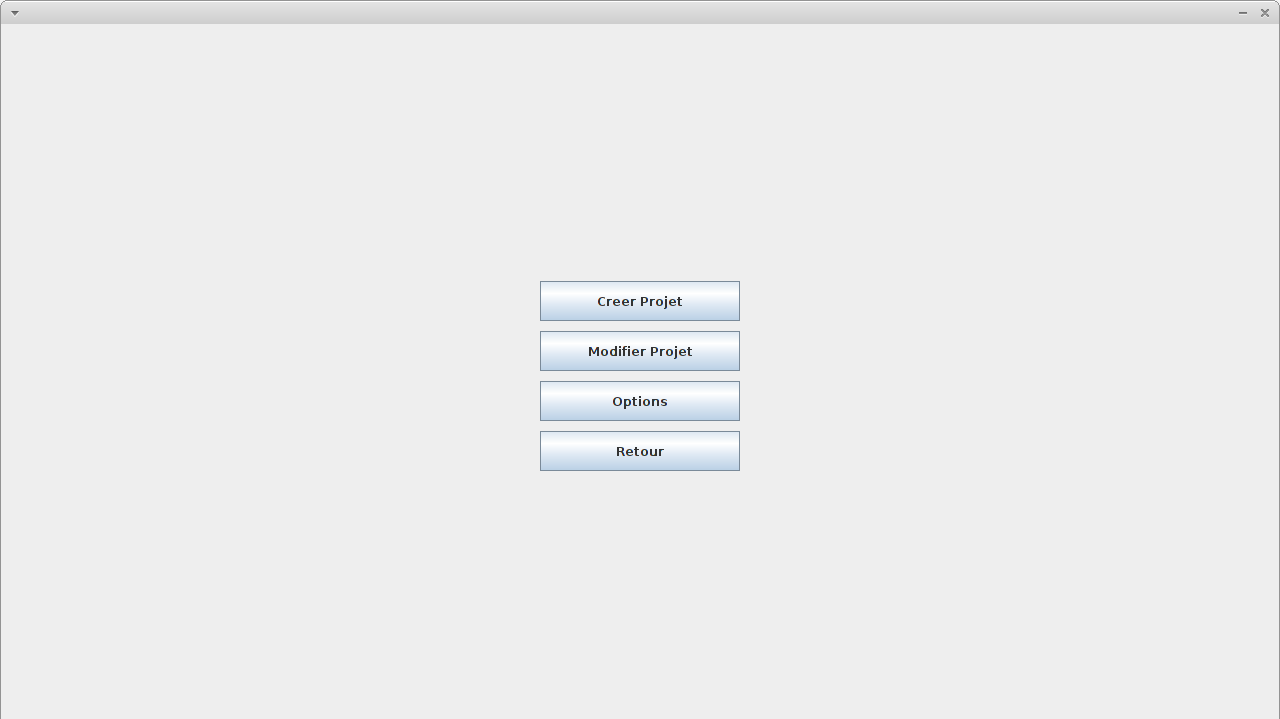
\includegraphics[scale=0.3]{IHM/selection_projet.png}
\caption{Ecran du menu administrateur}
\end{figure}
\begin{figure}
\centering
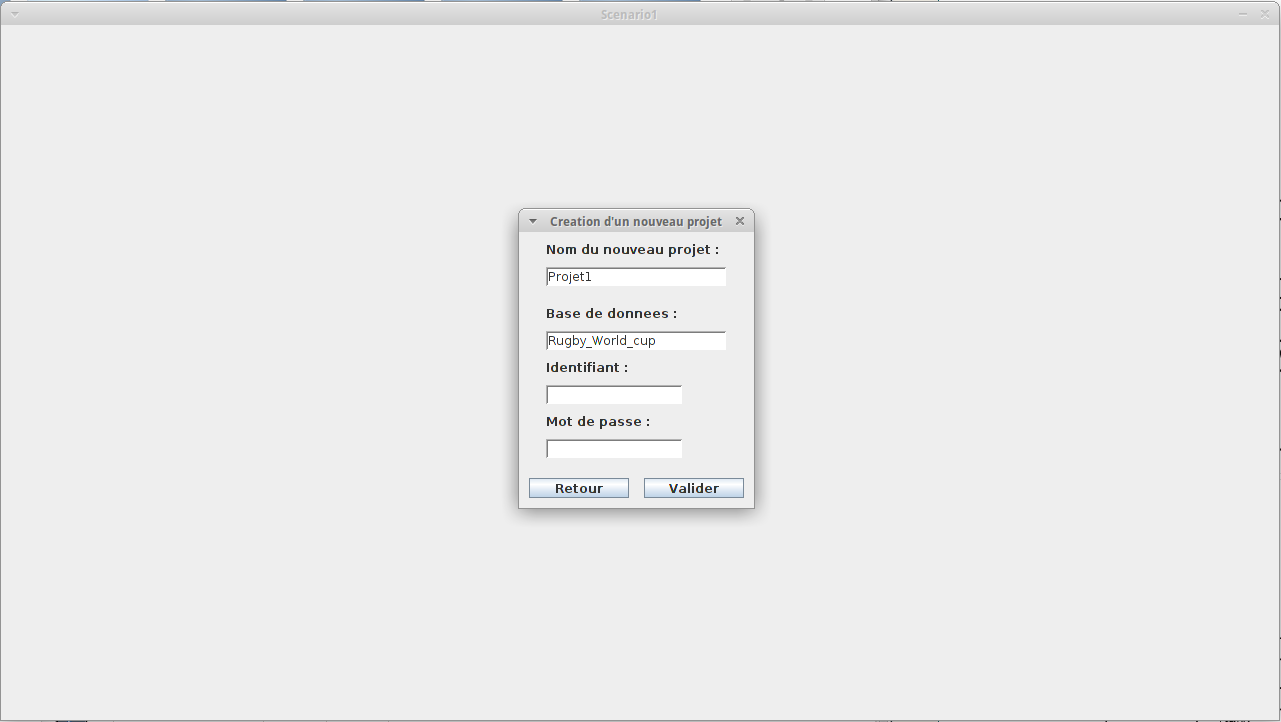
\includegraphics[scale=0.3]{IHM/creation_projet.png}
\caption{Ecran de création d'un nouveau projet}
\end{figure}
\begin{figure}
\centering
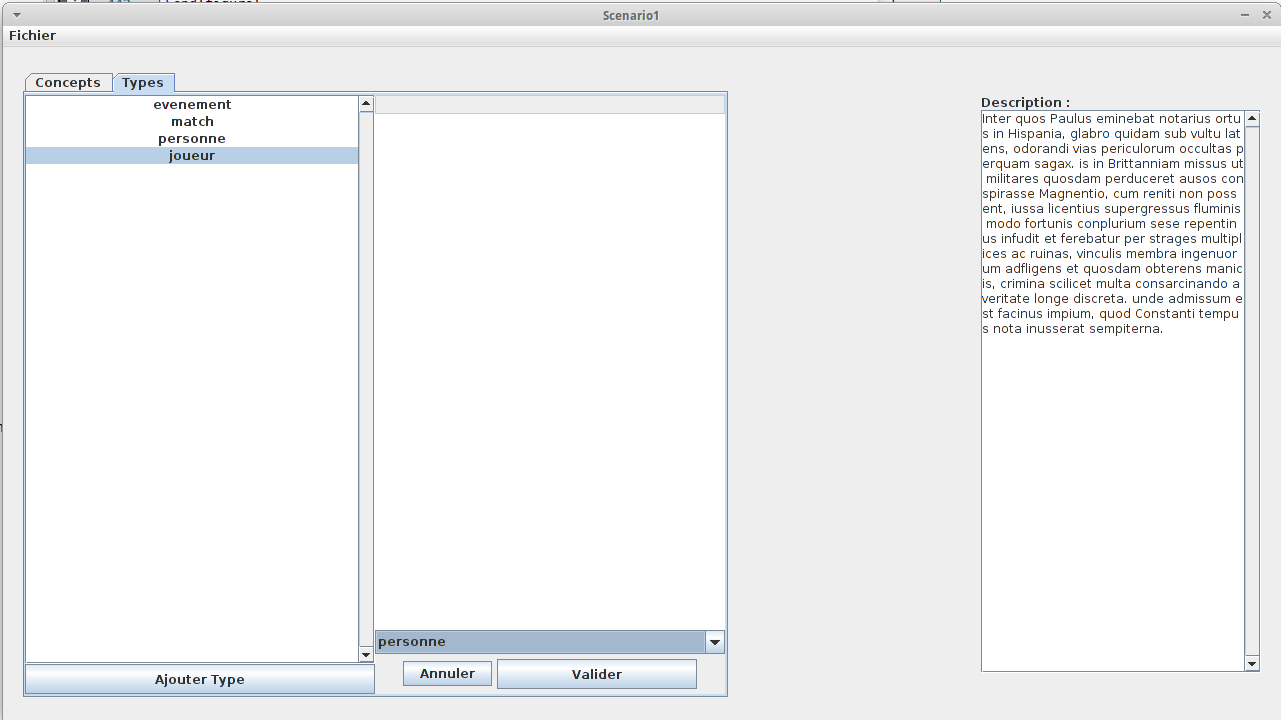
\includegraphics[scale=0.3]{IHM/creation_types.png}
\caption{Ecran de création des types}
\end{figure}
\begin{figure}
\centering
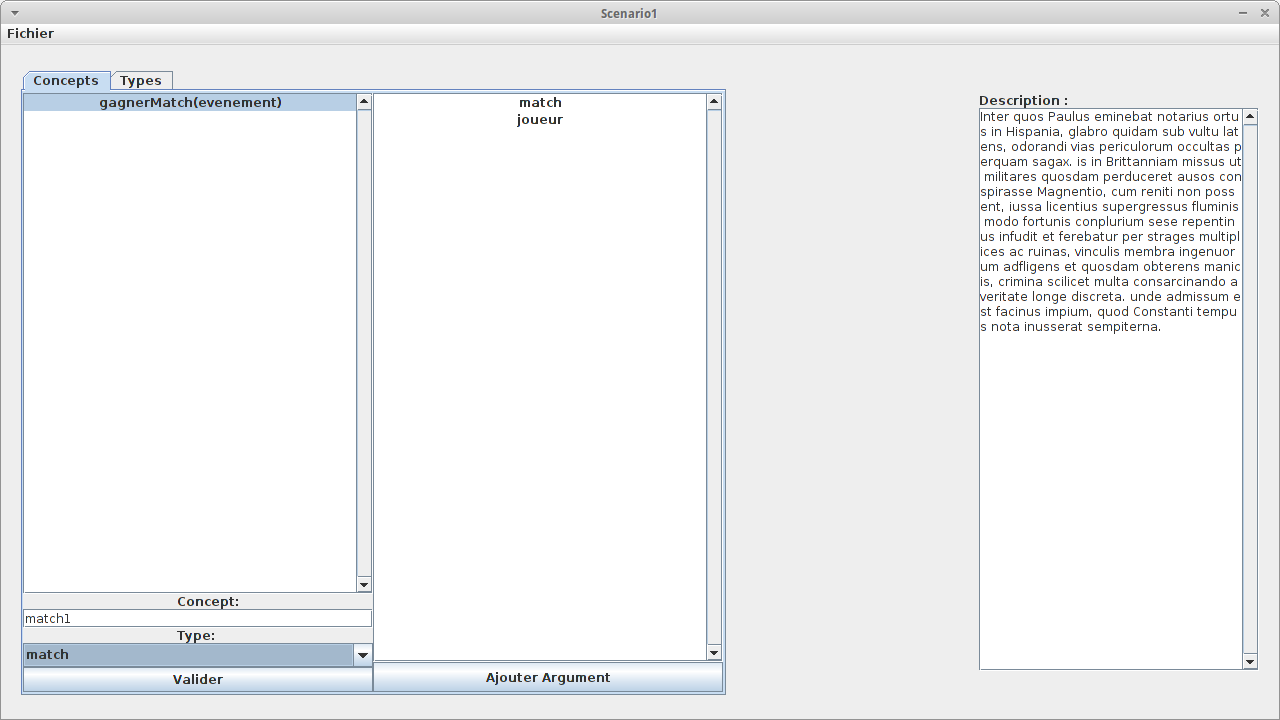
\includegraphics[scale=0.3]{IHM/creation_concepts.png}
\caption{Ecran de création des concepts}
\end{figure}
\begin{figure}
\centering
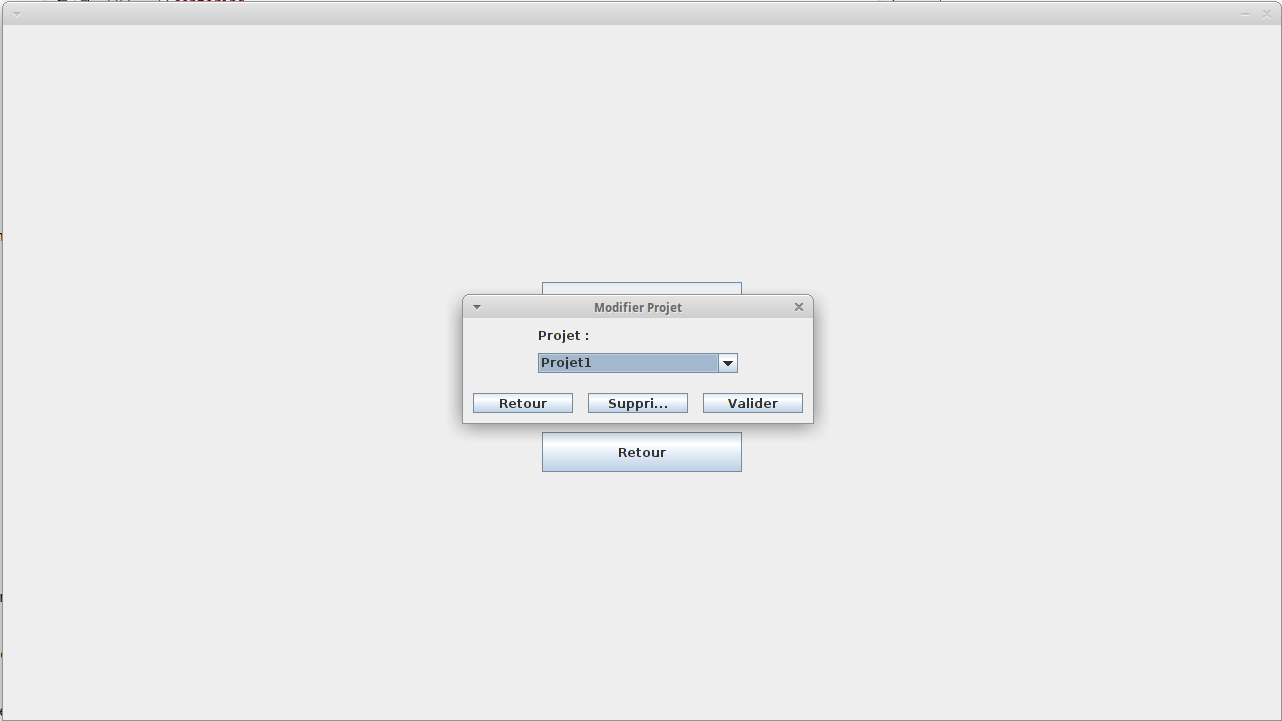
\includegraphics[scale=0.3]{IHM/modifier_projet_admin.png}
\caption{Ecran de choix du projet à modifier}
\end{figure}
\begin{figure}
\centering
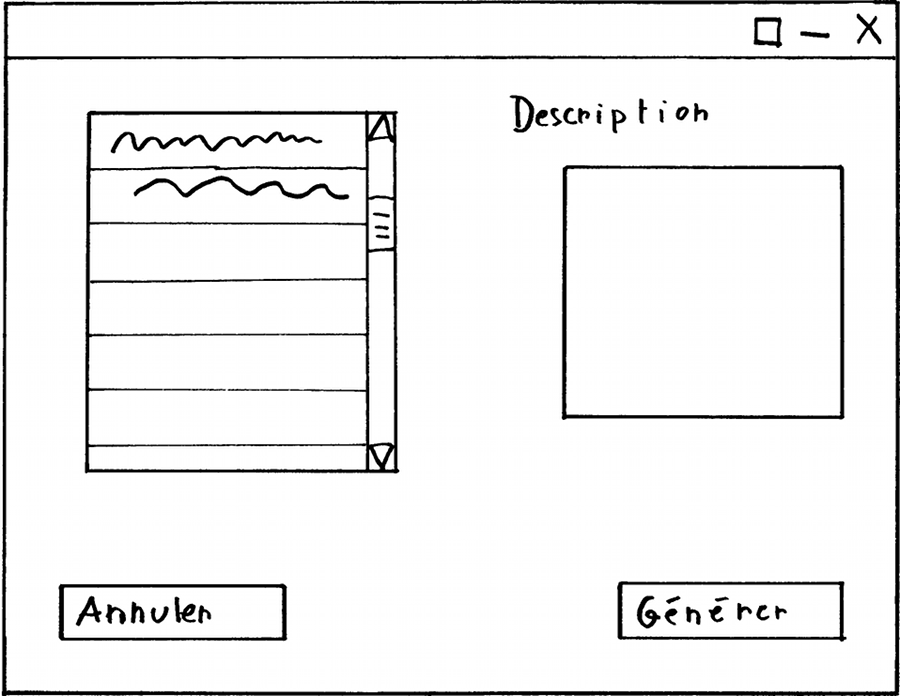
\includegraphics[scale=0.25]{Generation.png}
\caption{Ecran de choix des attributs}
\end{figure}

\chapter{Tests et résultats}
\section{Tests effectués}
Le but de ces tests est d'assurer le bon fonctionnement de notre application. Nous pouvons les regrouper selon l'ensemble de fonctionnalités auquels ils se rattachent. Afin de ne pas mélanger le code source et les essais, nous avons créé un package différent regroupant l'ensemble des classes et méthodes de test. 

\subsection{Package Linguistique}
Ce package regroupe les principaux objets utilisés par l'interface graphique tels que les concepts, graphes, noeuds et système de typage des concepts. Son bon fonctionnement était donc primordial pour ne pas avoir d'erreurs lors de l'utilisation de ces derniers par l'interface graphique. Nous avons donc élaboré des tests unitaires, au moyen de JUnit, sur chacune des classes et méthodes. 
\begin{itemize}	
\item ConceptTest : Permet de tester les classes Concept(Abstract/Complex/Simple). Dans ces classes nous avons majoritairement des accesseurs mais également des méthodes utilisées pour la génération de l'entrée Syntox. Notons que les accesseurs ne sont normalement pas des éléments soulevant des problèmes. Toutefois nous nous sommes assurés que les éléments retournés sont bien ceux attendus, surtout dans le cas de la liste et du nombre d'éléments qu'elle contient.
Concernant la méthode generateSyntox() nous avons choisi de la tester plus tard dans une autre classe qui utilise une méthode identique mais depuis un objet "GraphConcepts" et qui fait appel à cette méthode.
\item TypeTest : Permet de tester la classe TypeImpl qui implémente Type. Nous avons ici testé de manière similaire à "ConceptTest" les accesseurs présents en plus de la méthode "equals" dont nous avions besoin. 
\item TypeTreeTest et TypeTreeNodeTest : Les tests présents dans ces classes se rapportent respectivement aux classes du même nom, TypeTree et TypeTreeNode. Comme nous l'indiquent les commentaires, ces dernières permettent de représenter sous forme d'arbre, l'organisation et les liaisons des différents types.
Nous avons fait le choix de tester l'intégralité des méthodes présentes dans ces classes, à savoir :
	\begin{itemize}
	\item L'ajout d'un nouveau concept à la liste du noeud en question. 
	\item L'ajout d'un fils à la liste concernée.
	\item L'ajout d'un type dans l'objet TypeTree (Plus précisément dans la Map de l'objet) en respectant les liaisons avec un type prédécesseur (surType). De façon similaire, l'ajout d'un concept à ce même objet.
	\item La méthode permettant de retourner l'ensemble des sous-types que contient un type. 
	\end{itemize}
\item TypeManagerTest : Se rapporte à la classe TypeManager du package permettant de gérer la création des types ainsi que leur insertion dans l'arbre. 
Elle présente deux méthodes, différenciées par leurs arguments, permettant l'ajout d'un type dans l'arbre (makeType()). Nous les avons tout deux testées ainsi que la méthode retournant si deux types sont compatibles (isCompatible()).
\item LinguisticFactoryTest : Test de la classe LinguisticFactory (Singleton) qui permet la création d'un TypeManager. 
Nous avons choisi de tester les méthodes qui apportent les fonctionnalités suivantes: 
	\begin{itemize}
	\item L'ajout d'un type au TypeManager au moyen de sa propre méthode (makeType). Il a fallu faire de même que pour TypeManagerTest, c'est-à-dire tester les deux méthodes permettant cette fonctionnalité malgré que leur seule différence (les éléments pris en argument). 
	\item L'ajout de concept, simple ou complex à l'arbre qu'utilise le TypeManager. Ici aussi, nous avons réalisé deux tests selon la forme du concept. 
	\end{itemize}
\item GraphConceptsTest et GraphNodeDefault: GraphConceptsInterface et GraphNode sont des interfaces que les classes respectives GraphConcepts et GraphNodeDefault implémentent.
Ces classes permettent la représentation sous forme de graphe des concepts utilisés et sélectionnés par l'utilisateur au moyen de l'interface graphique. 
Nous avons testé pour ces classes :
	\begin{itemize}
	\item Certains accesseurs qui nous semblaient importants dans le sens où ces classes utilisent de nombreux objets d'autres classes, il est donc nécessaire de pouvoir garantir l'accès à ces objets et à leur référence. 
	\item La méthode permettant la création de la requête qui sera envoyée à Syntox (generateSyntox()). Cette méthode est appelée depuis GraphConcepts et fait appel à son homologue présente dans GraphNodeDefault.
	\end{itemize}
\end{itemize}
\subsection{Core}
	Dans ce package se trouvent toutes les classes permettant le lancement de notre application et les outils nécessaires tel que les éléments permettant la gestion de la sauvegarde des projets, un utilitaire regroupant les informations nécessaires pour la base de données et un système de cryptage/décryptage de mot de passe pour sécuriser l'accès à la base de données. 
Nous avons choisi de tester particulièrement les classes présentes dans les fichiers PasswordManager.java, Project.java et InfoDB.java. Plus précisément nous avons validé les fonctionnalités suivantes :
	\begin{itemize}
	\item L'encryptage ainsi que le décryptage d'un mot de passe. En effet, comme indiqué dans le cahier des besoins, nous ne souhaitons pas laisser le mot de passe utilisé pour la connexion à la base de données en clair. Il nous a donc fallu crypter une fois la connexion faite mais également décrypter si on doit réutiliser le mot de passe.
	\item La conservation des informations saisies pour la base de données au moyen de l'objet initBase. 
	\item L'ajout et la suppression de scénarios relatifs à un Projet.
	\end{itemize}
\subsection{Database[Connection/Inspection]}
\subsection{Syntox}

\subsection{Mémoire et temps de calcul}
	
\section{Résultats}

\chapter{Conclusion et perspectives}


\bibliographystyle{plain}
\bibliography{biblio}

\end{document}
